
%% Template Elsevier for Neuroimage

%% Use the option review to obtain double line spacing
%\documentclass[authoryear,preprint,review]{elsarticle}
\documentclass[authoryear]{elsarticle}
%\usepackage[framed,numbered,autolinebreaks,useliterate]{mcode}
\usepackage[framed,autolinebreaks,useliterate]{mcode}
\usepackage{natbib}
\usepackage{amsmath}
%\usepackage{lineno}
\usepackage{rotating}

\usepackage{hyperref}
\usepackage{amssymb}
\usepackage{amsfonts}


%\usepackage{algorithm2e}
%\usepackage{algorithmic}
%\usepackage{todonotes}
\usepackage{pdflscape}
\journal{Neuroimage}
\usepackage{color,transparent}
%\usepackage{color} 
%\pdfoptionpdfminorversion 6
\pdfminorversion=5

%\usepackage{graphicx}
%\usepackage{subcaption}
%\usepackage{mwe}
\usepackage{subfig}
\usepackage{caption}
%\usepackage{subcaption}
\usepackage{setspace}
\usepackage{lineno}
\usepackage{multirow}
\usepackage{array}
% Unique number for each line
\linenumbers
%\listoftodos
\newcommand\MyBox[2]{
  \fbox{\lower0.75cm
    \vbox to 1.7cm{\vfil
      \hbox to 1.7cm{\hfil\parbox{1.4cm}{#1\\#2}\hfil}
      \vfil}%
  }%
}

\renewcommand\arraystretch{1.5}
\setlength\tabcolsep{0pt}

\begin{document}

% Title must be 150 words or less
\begin{frontmatter}

%\title{Functional subtypes based prediction, a first step toward precision medecine}
\title{high-confidence prediction for high-risk diagnostic}

% Use letters for affiliations, numbers to show equal authorship (if applicable) and to indicate the corresponding author
\author[a,b]{Christian~Dansereau}
\author[c]{Angela~Tam}
\author[a,b]{Aman~Badhwar}
\author[c]{Sebastian~Urchs}
\author[a]{Pierre~Orban}
\author[a]{Pedro~Neto}
\author[a,b]{Pierre~Bellec}
\address[a]{Centre de Recherche de l'Institut Universitaire de G\'eriatrie de Montr\'eal, Montr\'eal, CA}
\address[b]{D\'epartement d'Informatique et de recherche op\'erationnelle, Universit\'e de Montr\'eal, Montr\'eal,CA}
\address[c]{Integrated Program in Neuroscience, McGill University, Montr\'eal,CA}
%

% Please keep the abstract between 250 and 300 words
\begin{abstract}
Alzheimer’s dementia (AD) is generally diagnosed based purely on the symptoms experienced by a patient. Post-mortem brain dissection studies have however established that this debilitating condition reflects heterogeneous neurobiological aberrations. To account for this heterogeneity, we developed a machine learning approach aimed at identifying a subgroup of subjects with homogeneous multimodal brain features, for which an accurate prediction of clinical diagnosis can be achieved. 

Method: 
We evaluated our approach by predicting clinical status in the ADNI2 sample, mixing control subjects and patients with AD [1]. A number of high-dimensional functional and structural biomarkers were generated for each individual: seed-based fMRI connectivity maps in 20 brain networks [3], surface-based cortical thickness measures across each hemisphere, as well as regional volume measures derived from the AAL parcellation [4]. 

We implemented a model to predict clinical diagnosis in the whole ADNI2 sample. This model first consisted of an unsupervised data dimension reduction step, for each biomarker taken independently. The dimension reduction started by computing the spatial similarity between maps across subjects, and applying a hierarchical clustering algorithm to identify subgroups with homogeneous maps. We computed the spatial correlation between each individual map and the average map per subgroup (called a subtype). These subtype weights were used to train a linear support vector machine model to predict clinical status. 

In a second stage, we trained a logistic regression classifiers to predict correct and incorrect classifications. In other words, we trained a classifier to tell which subjects could be confidently assigned to a clinical label, based on multimodal subtypes weights. We then computed separately the accuracy of prediction for subjects identified as “high-confidence prediction” vs “low-confidence prediction”. The full two-stage process was cross-validated using a ten-fold approach. The performance of the SVM was assessed separately for the “low confidence” and “high-confidence” cases in test data not used for training the model, thus providing unbiased accuracy estimates. 
 
Results  : 
In the full sample of 73 subjects (49 CN / 24 AD), the first level classification reached 79\%  accuracy. Out of those 73 subjects, 46 (34 CN / 14 AD) were identified as high-confidence. For those subjects alone, the classifier reached 89\% accuracy. For the remaining 27 low-confidence subjects (18 CN / 11 AD), the SVM classification only achieved 62\% accuracy (specificity 67\%, sensitivity 63\%). The model trained on CN and AD was then used to classify 79 MCI subjects at baseline. From that model, 10 subjects who showed an AD profile in the MCI population were identified with high-confidence. Looking at the longitudinal data it appeared that 9/10 of these subjects converted to AD between 5-37 months.

In the full sample of 68 subjects (48 control / 20 AD), the first level SVM classification reached 72.05\%  accuracy (specificity 74\%, sensitivity 72\%, f1 73\% and ROC AUC 0.81). Out of those 68 subjects, 39 (30 control / 9 AD) were identified as high-confidence. For those subjects alone, the classifier reached 89.7\% accuracy (specificity 90\%, sensitivity 90\%, f1 90\% and ROC AUC 0.94). For the remaining 29 low-confidence subjects (18 control / 11 AD), the SVM classification only achieved 48.3\% accuracy (specificity 52\%, sensitivity 48\%, f1 49\% and ROC AUC 0.56). 
 
Conclusions  : 
Our findings suggest that the participants of the ADNI2 samples have heterogeneous structural and functional brain features. Our approach demonstrates that machine learning model can be trained to recognize anatomo-functional markers for which a more accurate prediction of clinical diagnosis can be made. Finally our proposed approach revealed to be highly accurate to identify MCI converters up to 37 months prior to AD conversion.

\end{abstract}

%-- 
\begin{keyword}
High confidence \sep High risk \sep prediction accuracy \sep resting-state \sep fMRI connectivity
%fmri \sep effect size \sep multisite \sep clinical trial \sep AD biomarker
\end{keyword}
\end{frontmatter}

\section*{Highlights}

\begin{itemize}
\item TODO
\end{itemize}

\section{Introduction}
\paragraph{High-risk classification}
In many prediction task the impact of the decision may be important. lets think in the financial sector the decision to trade or not a stock may be very costly or in the case of healthcare the diagnostic of patient with  those applicaiton and many other are critical and therefore called high-risk predictions. We therefore would like to have some sort of confidence level for a given prediction based on prior knowledge of the performance of the trainned classification model and on the data given to the model in input.

For a classification task many factor may impact the performance of the model. The capacity of the prediction model, the quality of the input data and the discriminative information contained in it and finaly  ill defined labels.
\paragraph{Input data quality}
\paragraph{Capacity of the model}
In the case were the classification task is too complex for the capacity of the model the 

\paragraph{labels}

% Magic paragraph
\paragraph{Main objective}
Multisite studies are becoming increasingly common in resting-state functional
magnetic resonance imaging (rs-fMRI). In particular, some consortia have
retrospectively pooled rs-fMRI data from multiple independent studies comparing
clinical cohorts with control groups, e.g. normal controls in the 1000
functional connectome project (FCP) \citep{Biswal2010}, children and adolescents
suffering from attention deficit hyperactivity disorder from the ADHD200
\citep{ADHD200,Fair2012}, individual diagnosed with autism spectrum disorder in
ABIDE \citep{Nielsen2013}, individuals suffering from schizophrenia
\citep{Cheng2015}, or elderly subjects suffering from mild cognitive impairment
\citep{Tam2015}. The rationale behind such initiatives is to dramatically
increase the sample size at the cost of decreased sample homogeneity. The
systematic variations of connectivity measures derived using different scanners,
called site effects, may decrease the statistical power of group comparisons,
and somewhat mitigate the benefits of having a large sample size
\citep{Brown2011,Jovicich2016}. In this work, our main objective was to
quantitatively assess the impact of site effects on group comparisons in rs-fMRI
connectivity.


\paragraph{Specific objectives}
Our first objective was to characterize, using real data, the amplitude of
systematic site effects in rs-fMRI connectivity measures across sites, as a function
of within-site variance. We based our evaluation on images generated from
independent groups at 8 sites equipped with 3T scanners, in a subset
($N=345$) of the 1000 FCP. Our second objective was to evaluate the impact of
site effects on the detection power of group differences in rs-fMRI
connectivity, as a function of the amplitude of the group difference, sample
size, as well as the balancing of groups across sites. We implemented for this
purpose a series of Monte Carlo simulations, mixing synthetic data with real
data in the 1000 FCP sample. One interesting feature of the "1000 FCP" dataset is the presence of one large site of $\sim200$ subjects and 7 small sites of $\sim20$ subjects per site. We were therefore able to implement realistic scenarios following either a monosite or a multisite design (with 7 sites), with the same total sample size. Finally, we repeated the Monte-Carlo using a SVM instead of a GLM, and assessed the impact of site effects on prediction accuracy rather than statistical power.

\section{Method}

\subsection{Imaging sample characteristics}
The full 1000 FCP sample includes 1082 subjects, with images acquired over 33 sites spread across North America, Europe, Australia and China. As the 1000 FCP is a retrospective study, no effort was made to harmonize population characteristics or imaging acquisition parameters \citep{Biswal2010}. A subset of sites was selected based on the following criteria: (1) 3T scanner field strength, (2) full brain coverage for the rs-fMRI scan, and, (3) a minimum of 15 young or middle aged adult participants, with a mixture of males and females (4) samples drawn from a population with a predominant Caucasian ethnicity. In addition, only young and middle aged participants (18-46 years old) were included in the study, and we further excluded subjects with excessive motion (see next Section). The final sample for our study thus included 345 cognitively normal young adults (150 males, age range: 18-46 years, mean$\pm$std: 23.8 $\pm$5.14) with images acquired across 8 sites located in Germany, the United Kingdom, Australia and the United States of America. The total time of available rs-fMRI data for these subjects ranged between 6 and 7.5 min and only one run was available. See Table \ref{table_dataset} for more details on the demographics and imaging parameters at each site selected in the study.  The experimental protocols for all datasets as well as data sharing in the 1000 FCP were approved by the respective ethics committee of each site. This secondary analysis of the 1000 FCP sample was approved by the local ethics committee at CRIUGM, University of Montreal, QC, Canada.


\subsection{Preprocessing}
Each fMRI dataset was corrected for slice timing; a rigid-body motion was then estimated for each time frame, both within and between runs, as well as between one fMRI run and the T1 scan for each subject \citep{Collins1994}. The T1 scan was itself non-linearly co-registered to the Montreal Neurological Institute (MNI) ICBM152 stereotaxic symmetric template \citep{Fonov2011}, using the CIVET pipeline \citep{Ad-Dab'bagh2006}. The rigid-body, fMRI-to-T1 and T1-to-stereotaxic transformations were all combined to re-sample the fMRI in MNI space at a 3 mm isotropic resolution. To minimize artifacts due to excessive motion, all time frames showing a frame displacement, as defined in \cite{Power2012}, greater than 0.5 mm were removed and a residual motion estimated after scrubbing. A minimum of 50 unscrubbed volumes per run was required for further analysis (13 subjects were rejected). The following nuisance covariates were regressed out from fMRI time series: slow time drifts (basis of discrete cosines with a 0.01 Hz highpass cut-off), average signals in conservative masks of the white matter and the lateral ventricles (average Pearson correlation across all subjects is 0.242  between gray matter and white matter signals, and 0.031 between gray matter and ventricles signals) as well as the first principal components (accounting for 95\% variance) of the six rigid-body motion parameters and their squares \citep{Giove2009,Lund2006}. The fMRI volumes were finally spatially smoothed with a 6 mm isotropic Gaussian blurring kernel. A more detailed description of the pipeline can be found on the NIAK website\footnote{\url{http://niak.simexp-lab.org/pipe_preprocessing.html}} and Github\footnote{\url{https://github.com/SIMEXP/}}.




\subsection{Cross-validation}
A nested cross-validation was performed for accuracy estimation and parameters optimization using leave-one out cross validation in order to estimate the generalizability of the model. Nested inside that cross-validation loop 10 fold crossvalidation was perform to search for the optimal hyperparameter of the models. 

\subsection{Subtypes}
Instead of performing our classification on a correlation matrix we introduce a new metric called subtype weights that is computed as follow:
For each network, we identified 10 subgroups by grouping subjects with similar FC maps through hierarchical agglomerative clustering resulting in subtypes template. We then derived subtype weights for each individual using the spatial correlation of the individual FC map and each subtype template. This dimensionality reduction show the degree of association for an individual connectivity map with the corresponding subtypes templates.


%\subsection{Two-steps classification}
\subsection{Confidence supervisor}


fist step
In this work we whanted to evaluate a given classification model performance and generalizability with respect to a dataset. To do so we first randomly cross-validate a model (in this case an svm classifier) with the trainning set and then compiled the results against the true labels resulting in  hit and miss labels. On average the number of hit predicted for a given sample will give an estimate of the probability of a hit for each subjects from the trainned classification model. Since the objective is to predict the labels of a subset of suject with high confidence we will only select the hit that show a very high probability (99\% hit). The hit/miss vector can be represented like a one-hot encoder and show the hit/miss for each class resulting in N vectors of the original size of the trainning vector y.

Second step
Iterate on the probability of a hit from the model
The second step consist of estimating the hit/miss per class with a second classification model. The simplest representation of this using binary classifier is to use one binary classifier for each class or for more complex model using a joint model like a fully connected deep network with the number of class as the number of output.




Using the training set from the previously generated subtype weights, we first trained a logistic regression (LR) model \cite{Fan2008} for the classification of the clinical labels (LRC). Second, an other logistic regression model (LRHM) was trained to predict the hit (correct classification) and miss (incorrect classification) labels from the LRC, using the subtype weights as an input. We then used the test set to evaluate the prediction accuracy of the two subgroups (easy and hard to classify subjects) by deriving the accuracy score separately for the “easy” and “difficult” to classify cases.

\begin{figure*}[tbp]
\centering
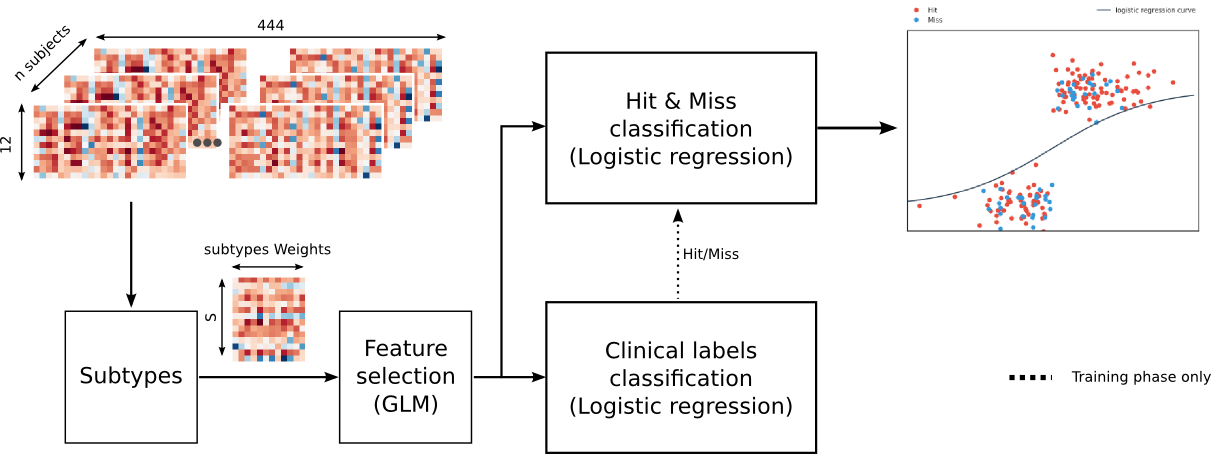
\includegraphics[width=\linewidth]{figures/full_model.png}
\caption{Caption}
\label{fig_model_schematic}
\end{figure*}

\subsection{Interpretation of the models coefficients}

\subsection{Association with phenotypic variables}


\paragraph{Public code and data}
The code used in this experiment is available on a 
GitHub repository at the following URL\footnote{\url{https://github.com/cdansereau/}}. A IPython Notebook is also provided with all of the figure generation scripts. The functional imaging data is publicly available on the NITRC web site\footnote{\url{http://fcon_1000.projects.nitrc.org/indi/retro/cobre.html}}.



\section{Results}

\subsection{Inter-site effects in fMRI connectivity}


\begin{figure}[htbp]
\begin{center}
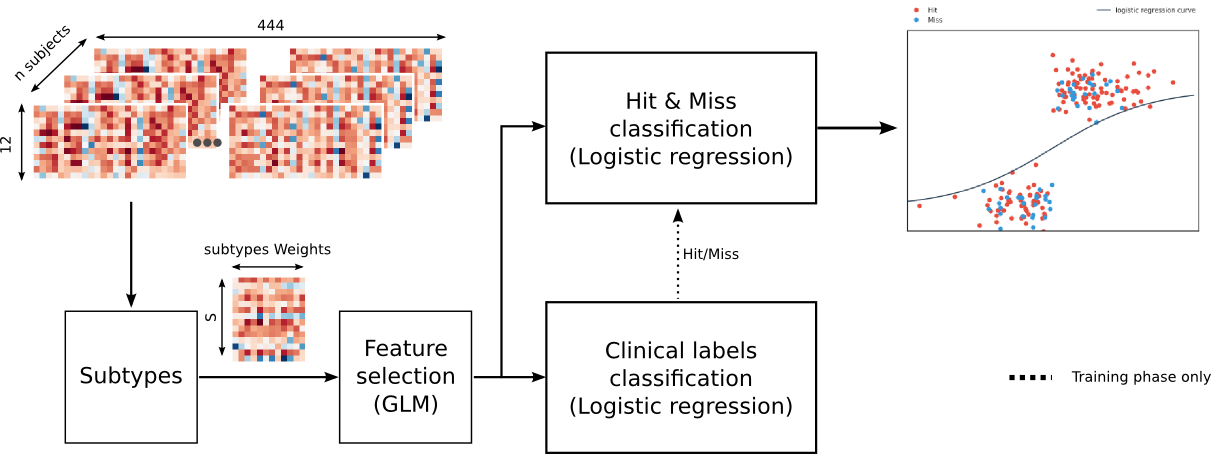
\includegraphics[width=0.8\linewidth]{figures/full_model.png}
\end{center}
\caption[DMN variability across sites]{
Panel A: map of the DMN obtained using a seed in the posterior cingulate cortex, averaging all subjects and sites together (first row) and then averaging all subjects for each of the 8 sites (subsequent rows). Panel B shows the number of sites with a significant inter-site difference for each brain region (first row) and the significant differences between the average functional connectivity maps of one site versus all the others (subsequent rows).
}
\label{fig_DMN_variability}
\end{figure}

\begin{table}[htbh]
\center
\caption{\small{Summary results with no split. The accuracy is 71.3\%}}
\label{my-label}
\begin{tabular}{lllll}

\textit{Class} & \textit{precision} & \textit{recall} & \textit{f1-score} & \textit{support} \\ \hline
0         & 78\%      & 69\%   & 73\%     & 58      \\
1         & 64\%      & 74\%   & 69\%     & 43      \\ \hline
avg/total & 72\%      & 71\%   & 71\%     & 101     \\ \hline
\end{tabular}
\caption{\small{Summary results with split on the right. The accuracy is 79.2\%}}
\label{my-label}
\begin{tabular}{lllll}

\textit{Class} & \textit{precision} & \textit{recall} & \textit{f1-score} & \textit{support} \\ \hline
0         & 81\%      & 88\%   & \textbf{85\%}     & 34      \\
1         & 75\%      & 63\%   & 69\%     & 19      \\ \hline
avg/total & 79\%      & 79\%   & 79\%     & 53     \\ \hline
\end{tabular}
\caption{\small{Summary results with split on the left. The accuracy is 62.5\%}}
\label{my-label}
\begin{tabular}{lllll}

\textit{Class} & \textit{precision} & \textit{recall} & \textit{f1-score} & \textit{support} \\ \hline
0         & 71\%      & 42\%   & 53\%     & 24      \\
1         & 59\%      & 83\%   & 69\%     & 24      \\ \hline
avg/total & 65\%      & 60\%   & 61\%     & 48     \\ \hline
\end{tabular}
\end{table}



%%%%%%%%%%%%%%%%%%%%%%%%%%%%%%%%%%%%%%%%%%%%%
% END of results section                    %
%%%%%%%%%%%%%%%%%%%%%%%%%%%%%%%%%%%%%%%%%%%%%

\section{Discussion and conclusions}

\paragraph{Inter-site effects in rs-fMRI connectivity} 


\section{Acknowledgments}
Parts of this work were presented at the 2013 annual meeting of the Organization for Human Brain Mapping, as well as the 2013 Alzheimer's Association International Conference (AAIC) \citep{Dansereau2013b}. The authors are grateful to the members of the 1000 functional connectome consortium for publicly releasing their datasets. The computational resources used to perform the data analysis were provided by ComputeCanada\footnote{\url{https://computecanada.org/}} and CLUMEQ\footnote{\url{http://www.clumeq.mcgill.ca/}}, which is funded in part by NSERC (MRS), FQRNT, and McGill University. This project was funded by NSERC grant number RN000028 and the Canadian
Consortium on Neurodegeneration in Aging (CCNA), through a grant from
the Canadian Institute of Health Research and funding from several partners including SANOFI-ADVENTIS R\&D. PB is supported by a salary award from ``Fonds de recherche du Qu\'ebec -- Sant\'e'' and the Courtois Foundation.

\section*{References}

\bibliographystyle{elsarticle-harv}
\bibliography{biblio}


\pagebreak



\clearpage
\appendix


%% SUPPLEMENTARY MATERIAL
\clearpage
\pagebreak
\renewcommand{\thefigure}{S\arabic{figure}}
\renewcommand{\thetable}{S\arabic{table}}
\setcounter{figure}{0}
\begin{center}
\emph{Supplementary Material {--} Statistical power and prediction accuracy in multisite resting-state fMRI connectivity}\\

\vspace{\baselineskip}Submitted to Neuroimage.\\

\vspace{\baselineskip}C. Dansereau$^{1,2}$,  Y. Benhajali$^{1,3}$,C. Risterucci$^{4}$, E. Merlo Pich$^{4}$, P. Orban$^{1}$, D. Arnold$^{5}$, P. Bellec$^{1,2}$\\

\end{center}

$^1$Centre de Recherche de l'Institut Universitaire de G\'eriatrie de Montr\'eal, Montr\'eal, CA\\
$^2$Department of Computer Science and Operations Research, University of Montreal, Montreal, CA\\
$^3$D\'epartement d'anthropologie, Universit\' de Montr\'eal, Montr\'eal, CA\\
$^4$Clinical Imaging, pRED, F.Hoffman-La Roche, Basel, CH\\
$^5$NeuroRx inc., Montr\'eal, CA\\

For all questions regarding the paper, please address correspondence to Pierre Bellec, CRIUGM, 4545 Queen Mary, Montreal, QC, H3W 1W5, Canada. Email: pierre.bellec (at) criugm.qc.ca.\\




\end{document}


